\documentclass[pageno]{jpaper}
\usepackage[english]{babel}
\usepackage[normalem]{ulem}
\usepackage{pifont}
\usepackage{mathtools}
\usepackage{listings}
\hypersetup{
     colorlinks   = true,
     citecolor    = black,
     linkcolor    = black
}

%\numberofauthors{2}

\begin{document}

\title{Exploiting Approximation to Accelerate Distributed Training of Neural Networks}

\DeclareRobustCommand{\authorthing}{
\begin{tabular}[t]{cc}
Sandeep D'Souza & Vignesh Balaji & Nandita Vijaykumar \\
\texttt{sandeepd@andrew.cmu.edu} & \textt{vigneshb@andrew.cmu.edu} & \texttt{nandita@cmu.edu}\\
\multicolumn{3}{c}{\textbf{Carnegie Mellon University}}
\end{tabular}
}
\author{\authorthing}

\date{}
\maketitle
\let\oldtabular\tabular
\renewcommand{\tabular}{\footnotesize\oldtabular}

\thispagestyle{empty}

\begin{abstract}

The increase in the amount of data used by machine learning
applications has necessitated the need for distribution across
many machines. Distribution at this scale poses a challenge
to efficiently scale computations across multiple workers.
In the context of distributed training of deep neural networks, 
synchronous updates every iteration restricts scalability to
a few machines. To address this scalability bottleneck, we 
exploit the tolerance of neural networks to approximations.
We explore different approximation strategies that elide
updates to the different layers of the network.
Our studies reveal that approximating updates to a few 
layers of the neural network can improve the training
time of the network without significantly compromising
the accuracy of the trained model.



\end{abstract}




\section{Introduction}
Deep Neural Networks constitute a state-of-the-art technique across many domains which use machine learning such as autonomous cars, speech recognition, image/video processing, etc. These neural networks however require training over massively large datasets. Hence, training these networks has become notoriously difficult, requiring a significant amount of computational resources to complete in a reasonable amount of time. Traditional formulations of neural networks focus on serialized implementations, which in practice take a very long time to train. In order to overcome this shortcoming a lot of work has focused on parallelizing some aspects of the training phase in order to obtain speedup training. Single node platforms with GPUs have been one of the key ways by which system designers have been able to speed up training. However, a single system cannot be used for large scale training on petabytes of data. It is essential that the training be split up over multiple distributed nodes. This has led to the development of large-scale distributed machine learning frameworks such as TensorFlow~\cite{tensorflow}. 

To test the scalability of distributed training, we performed a number of experiments using TensorFlow to perform the image classification task over the CIFAR-10~\cite{cifar10} dataset. Our experiments show that counterintuitively, scaling out across multiple does not provide the expected speedup in distributed training. A likely reason is the large amount of data that is exchanged over the network to keep the models that are trained in parallel consistent with each other, to ensure convergence. 

In this project, our goal is to accelerate distributed neural network training by leveraging the \emph{approximation-tolerant} nature of these algorithms. It is well known that neural networks are tolerant to towards different approximations that can be leveraged to speed up inference~\cite{x,y}, however, principled approximation in training has been largely unexplored. 

In this project we will focus on optimizing the training of deep neural networks from a systems perspective.
We will explore how approximation can help reduce training time without sacrificing accuracy. The project
is highly relevant to the course and would focus on a number of concepts covered in the course, such as
consistency and distributed computation models


\section{Background}


\section{Experimental Setup}
In this section we describe our experimental setup to evaluate the scalability of distributed training and investigate techniques to accelerate training by leveraging approximations. 
\subsection{TensorFlow}
TensorFlow (~\cite{tensorflow}) is a machine learning system that is designed to operate at large scale across numerous heterogeneous distributed systems. TensorFlow using dataflow graphs to represent the desired computation for a machine learning algorithm. TensorFlow allows distributing the computation between different nodes in a distributed system by replicating the dataflow graph across different nodes or partitioning subgraphs of the computation across different nodes. 

\subsection{Cifar10}
\subsection{Distributed System Infrastructure}

\section{Motivation} \label{sec:motivation}

In this section, we discuss the motivation for distributing
machine learning applications across different machines.
We then discuss our experiments to understand the effect of
synchrony on the performance and model accuracy of a distributed
deep neural network training task.

\subsection{Distributed Machine Learning}

Recent advances in AI tasks such as a speech recognition and visual 
object classification have been made possible by complex models
that operate on large amounts of data. Modern systems \cite{distbelief}
\cite{projectadam}\cite{parameterserver} develop large and complex
models with around a billion to trillion parameters. Handling data
at such scale is beyond the capability of any single machine. As a 
result, distributing the machine learning task across many different
machines has become a necessity. However, distributing work at 
this scale introduces new challenges.

Large scale distribution creates a communication bottleneck. Most 
machine learning applications are iterative algorithms that progressively
refine the result. The most intuitive form of parallelism for such 
applications is to divide the input data among many workers and 
synchronize the progress made by each worker every iteration. The 
problem with this Bulk Synchronous Parallelism model of distribution 
is that the barrier at the end of each iteration affects scalability.
The presence of even a few stragglers (workers that take more time
to complete an iteration relative to other workers in a system) 
has a huge performance penalty on the application.

The problem of stragglers has spawned active research on a variety
of consistency models that relax synchronization without compromising
the convergence rate\cite{communicationthesis}\cite{gangerstraggler}.
We performed experiments to understand the effect of synchronization 
on the execution time and model accuracy of disrtibuted training.

\subsection{Effect of Synchronization}

\begin{figure}[h]
\centering
  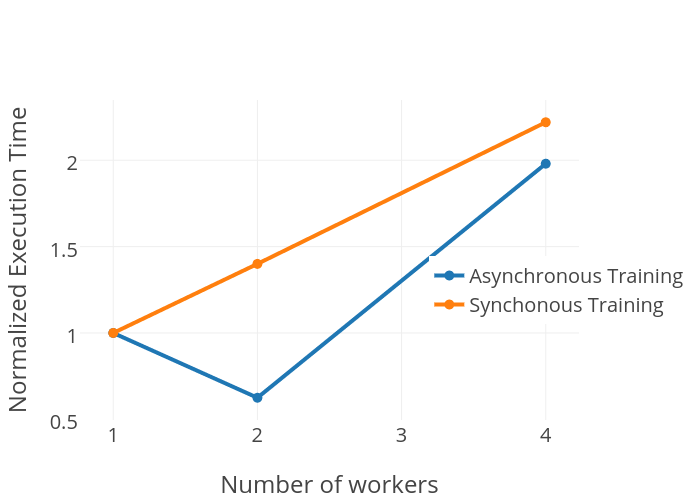
\includegraphics[keepaspectratio,width=.9\columnwidth]{figures/15712-corrected-scalability.png}
  \caption{\textbf{Scalability to multiple workers}}
  \label{fig:scalability}
\end{figure}

Figure \ref{fig:scalability} shows the execution time required 
to complete 20000 steps when run with 1,2 and 4 workers with
and without synchronization. The 
execution times for all the configurations are normalized to 
the single worker case. The data shows that the performance
of the precise and execution 





> Why distribute? 
Model parallelism allows training more complex models with many 
parameters. This is a progression from using GPUs to many different
machines. 

> synchronous training scalability. Impact of synchrony on accuracy
Why do we use synchronous training. Is it because we have a system
that is similar to the single node version? 
This berkeley thesis talks about why synchronization is important. 
Apparently synchronization allows for faster convergence because 
the average of the local updates of different machines reduces the
variance in data which leads to faster convergence. (https://www2.eecs.berkeley.edu/Pubs/TechRpts/2016/EECS-2016-47.pdf)
Blindly removing synchrony in an application does not seem to be
completely useful.

The impact of asynchrony on accuracy is that we are making judgements
on only part of the data that was present in our local store. This
higlights the dependence of the distribution of data and the homogeniety
(in terms of information) of the data. I think this was the premise of 
the hogwild paper.

> How does asynchrony affect training time? And accuracy
Stragglers are an issue in any large scale distributed training. If 
we use machines with different processing times (as in a distributed
cluster with different processing times) then the effects of stragglers
are exaggerated. 





\section{Leveraging heterogeneous approximation to accelerate distribute training}
\section{Hypotheses}

\section{Evaluation and Analysis}
In this section, we evaluate the above techniques to leverage the approximation-tolerance of the neural network to accelerate distributed training. We essentially perform \textit{training update elisions}, which involves not updating the weights and biases of specific layers at certain training steps. Two kinds of training elisions were explored:
\begin{itemize}
	\item \textit{Periodic Training Elision} involves performing training elisions once every $n$ steps, where $n$ is called the periodic elision interval. The parameters of the entire network are updated for $n-1$ steps, followed by a step where only parameters corresponding to certain layers are updated.
	\item \textit{Selective Early Termination} involves training the entire network until a given training step $\kappa$. For steps after $\kappa$, only parameters corresponding to certain layers are updated, while updates and gradient computation for other layers are elided.

\end{itemize}

Both types of approximations partially update the model weights in a specified training step. We expect that using update elision will reduce the amount of computation required in a training step, as well as the communication overhead required for distributed training. 

We now discuss the experimental results. Different approximation techniques are compared on the basis of classification accuracy (on the full testing data) and training time. We present results for both single node training as well as distributed training for a number of different cluster configurations. In each of our experiments, we checkpoint the model every 1000 trained steps, and use the checkpointed model to compute the achieved classification accuracy.

\subsection{Periodic Training Elision}
\subsubsection{Sensitivity of Different Layers to Training Elision}
To determine how the convergence of the model is impacted by the training elision for different layers, we conducted an experiment where we did not train or update a different number of layers every \emph{alternate step}. Figure~\ref{fig:fig1} depicts the accuracy achieved during training while periodically eliding training for a different number of layers starting from the bottom up (dashed lines) and top down (unbroken lines). 
\begin{figure}[t]
	\centering
	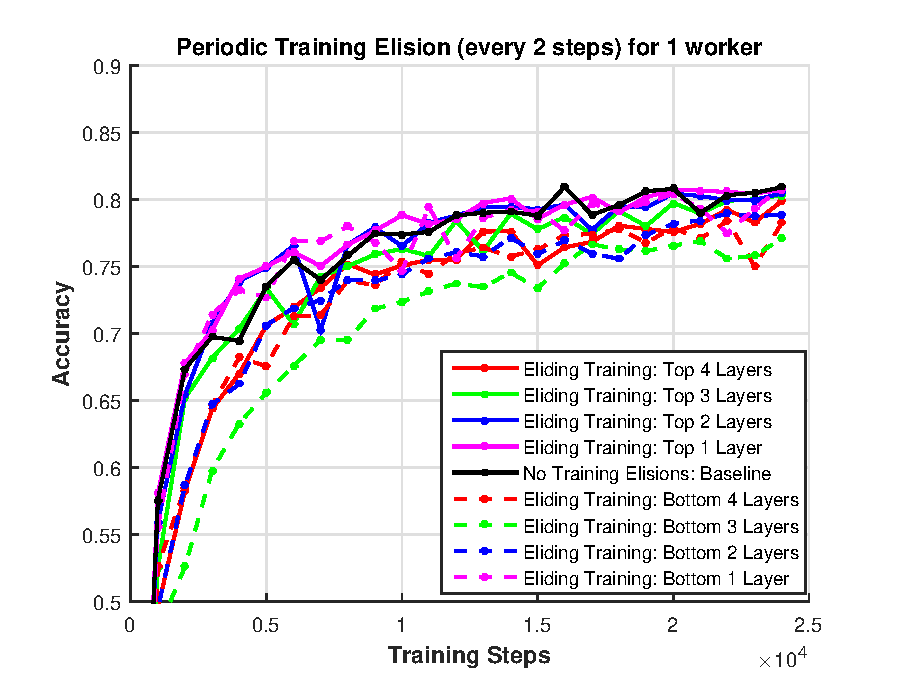
\includegraphics[width=0.8\columnwidth]{figures/fig1.eps}
	\caption{Periodic Training Elision (every 2 steps)}
	\label{fig:fig1}
\end{figure}
From Figure 1, we make the following observations: 
\begin{enumerate}
\item Eliding a single layer (top-most or bottom-most) has negligible impact on accuracy.
\item When eliding the \emph{same number} of layers, eliding training for the \emph{top layers} first consistently faster convergence and better accuracy than eliding the bottom layers.
\item Eliding the bottom 4 layers anomalously produces faster convergence than eliding the 3 bottom layers. 
\end{enumerate}
\subsubsection{Single Node Accuracy \& Training Time.}
In addition to Figure~\ref{fig:fig2} where the periodicity of training elision was \emph{two steps}, we conduct an experiment where we elide training at a periodicity of \emph{5 steps}. The accuracy results are depicted in Figure~\ref{fig:fig2}. We find that the neural network is resilient enough to tolerate this approximation irrespective of the number of layers for which training was elided with the exception of eliding the bottom 4 layers which produced a minor reduction in the accuracy. 
\begin{figure}[t]
	\centering
	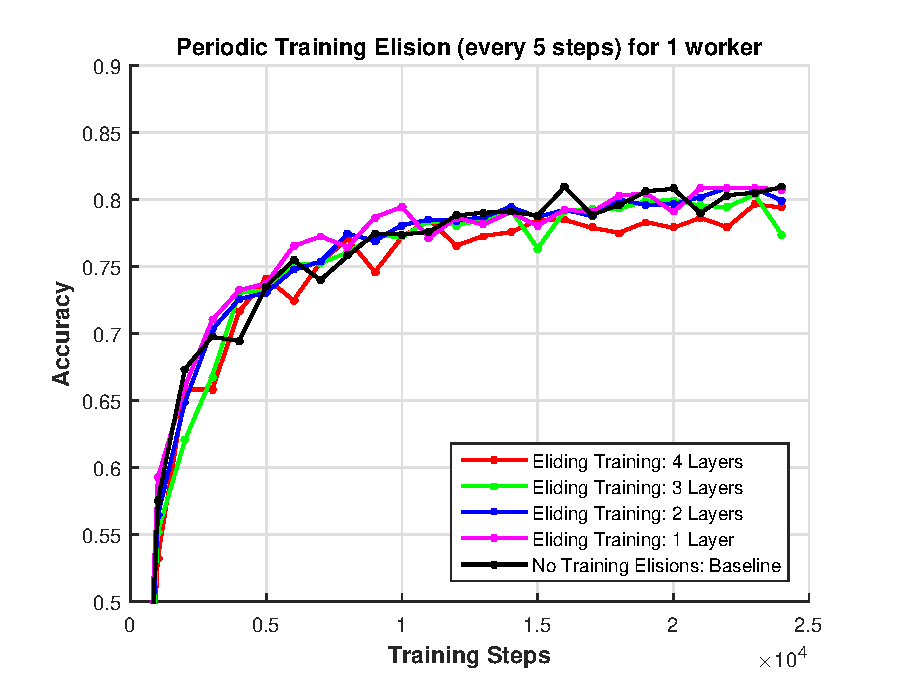
\includegraphics[width=0.8\columnwidth]{figures/fig2.eps}
	\caption{Periodic Training Elision (every 5 steps)}
	\label{fig:fig2}
\end{figure}
We also evaluated the resulting speedup in training time as a result of the described approximations. Figure~\ref{fig:fig3}depicts the normalized training speedup for both 2 and 5 step periodic training elision. We make the following observations: \emph{(i)} we observe that eliding training for 4 layers (2 step) produces a speedup of as much as 45\%; \emph{(ii)} Eliding training with a lower periodicity of 5 steps does not produce a significant bump in speedup (only 11.8\%); \emph{(iii)} Eliding a single layer produces only an insignificant improvement in training time. Since this is a single node experiment, the speedups come from eliding the gradient computation for several layers.  

\begin{figure}[t]
	\centering
	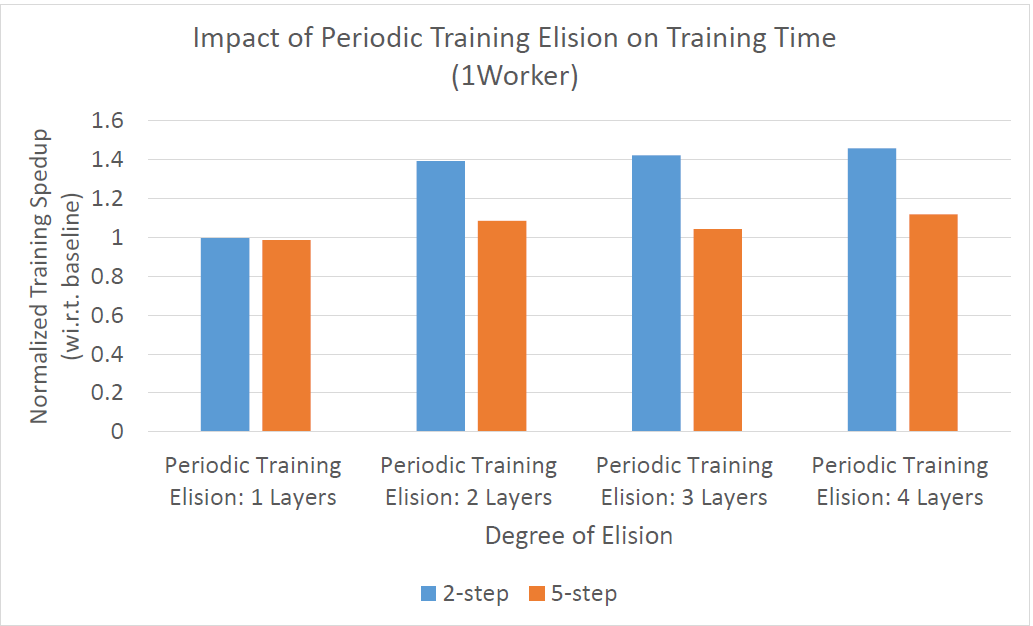
\includegraphics[width=0.8\columnwidth]{figures/fig3.PNG}
	\caption{Normalized speedup for Periodic Training Elision (every 2 and 5 steps)}
	\label{fig:fig3}
\end{figure}

%Figure 1: Periodic Training Elision (every 2 steps for both upper layers and lower layers) -- Accuracy
%Figure 2: Periodic Training Elision (every 5) -- Accuracy
%Figure 3: Periodic Training Elision (every 2 \& 5 steps for both upper layers and lower layers) -- Execution Time
\subsubsection{Mutiple Workers Accuracy and Training Time.}
Figure~\ref{fig:fig4} depicts periodic training elision in a distributed setting with 4 workers. We find that approximating training for both 3 and 4 layers does not have a noticeable impact on convergence or accuracy.\footnote{It is possible that the impact of approximation is only noticeable after our evaluated training time of 2000 steps.} Figure~\ref{fig:fig5} depicts the normalized speedup for periodic training elision with 4 workers. We find that periodic training elision is able to provide a speedup of as much as 2.7x while eliding training for 3 layers, and 2.85x for 4 layers. 

\begin{figure}[t]
	\centering
	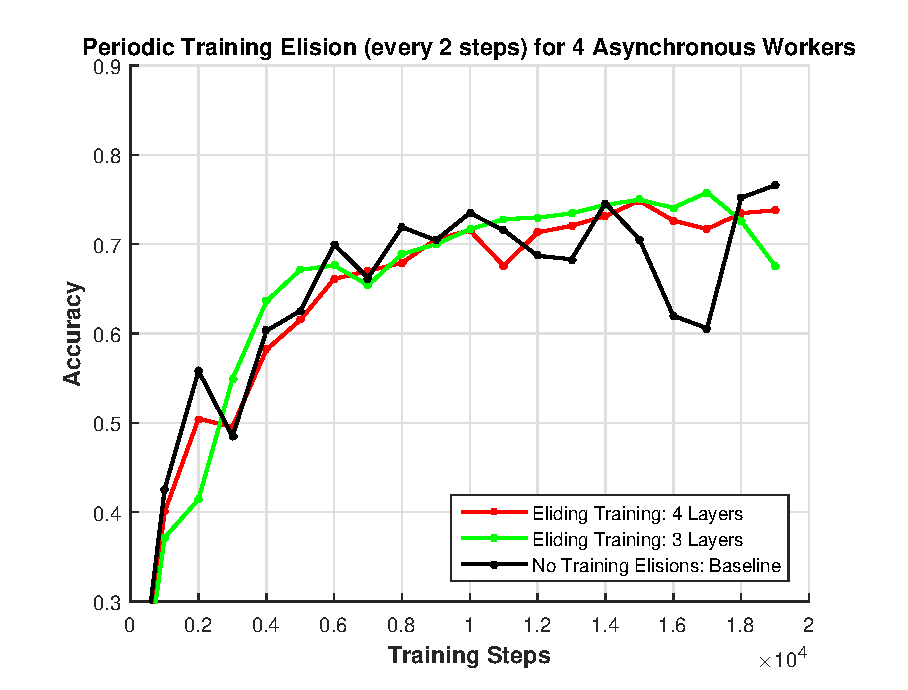
\includegraphics[width=0.8\columnwidth]{figures/fig4.eps}
	\caption{Periodic Training Elision: 4 workers (every 2 steps)}
	\label{fig:fig4}
\end{figure}

\begin{figure}[t]
	\centering
	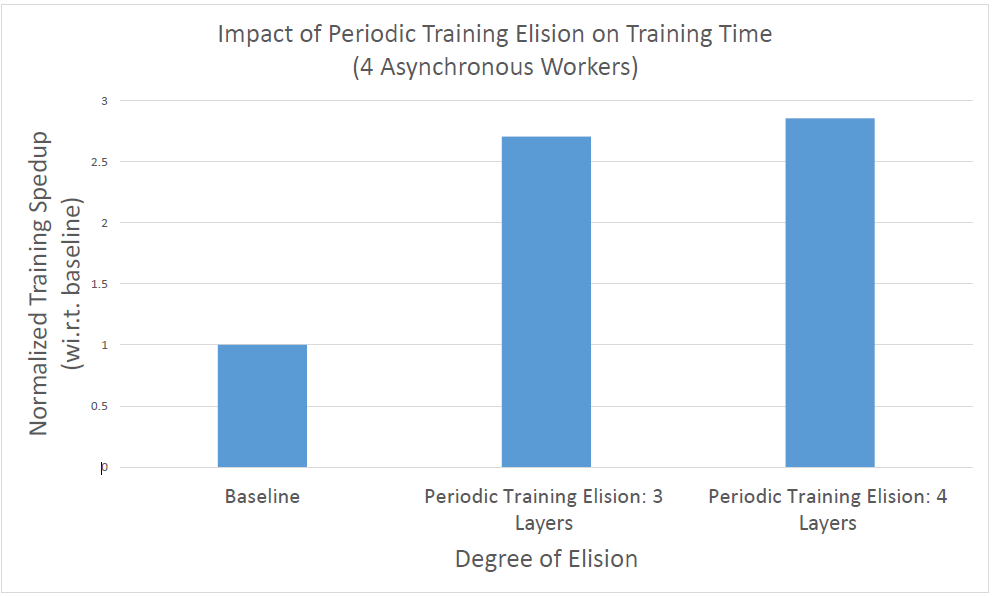
\includegraphics[width=0.8\columnwidth]{figures/fig5.PNG}
	\caption{Normalized speedup for Periodic Training Elision: 4 workers (every 2 steps)}
	\label{fig:fig5}
\end{figure}
%Figure 4: Periodic Training Elision 4 workers (every 2 steps for both upper layers and lower layers) -- Accuracy
%Figure 5: Periodic Training Elision 4 workers (every 2 steps for both upper layers and lower layers) -- Execution Time
\subsection{Selective Early Termination}
\subsubsection{Single Node Accuracy and Speedup} 
In Figure~\ref{fig:fig6}, we plot the obtained accuracy versus the training step for a selective early termination experiment running on a single machine. For each of the compared experiments we train all layers of the model until the 5000th training step. For the subsequent steps the training data is used to update only the top $\eta$ trainable layers of the model, where $\eta$ was chosen between $1$ to $4$ in our experiments. Note that, for a $N$ layer neural network $\eta=i$ corresponds to update elision for the first $N-\eta$ trainable layers. From the plot we can observe that eliding one layer has a neglible impact on accuracy, but eliding more than one layer leads to about 3\% drop in accuracy. After the training termination point, the network continues to improve accuracy for a short while, before converging on accuracy that is less than Baseline. 
Figure~\ref{fig:fig7} depicts the normalized speedup for selective early termination. We find that on a single machine selective early termination is able to produce as much as 2.3x reduction in training time.  

\begin{figure}[t]
	\centering
	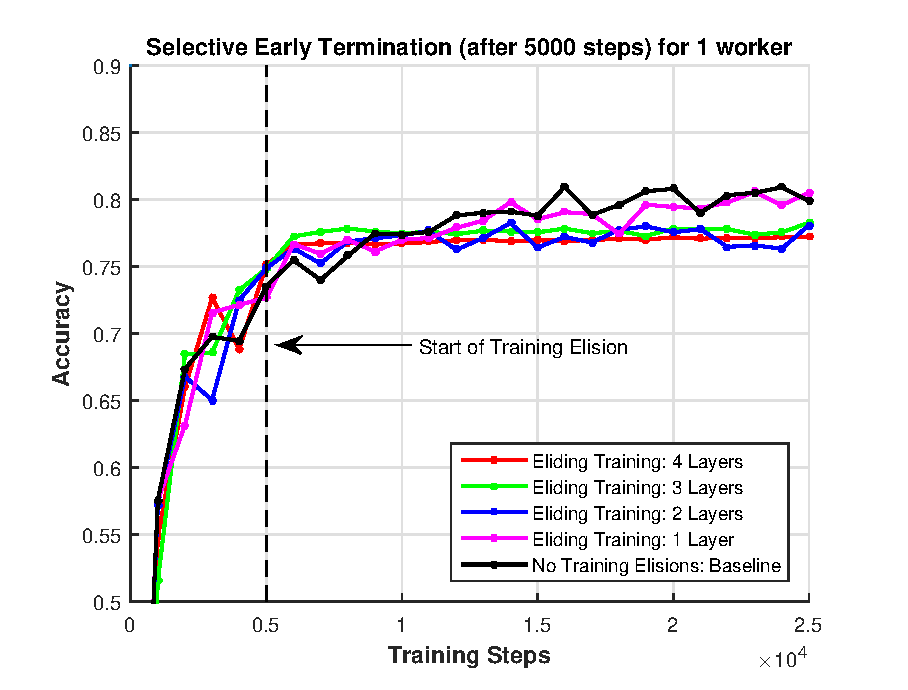
\includegraphics[width=0.8\columnwidth]{figures/fig6.eps}
	\caption{Selective Early Termination: 1 worker}
	\label{fig:fig6}
\end{figure}

\begin{figure}[t]
	\centering
	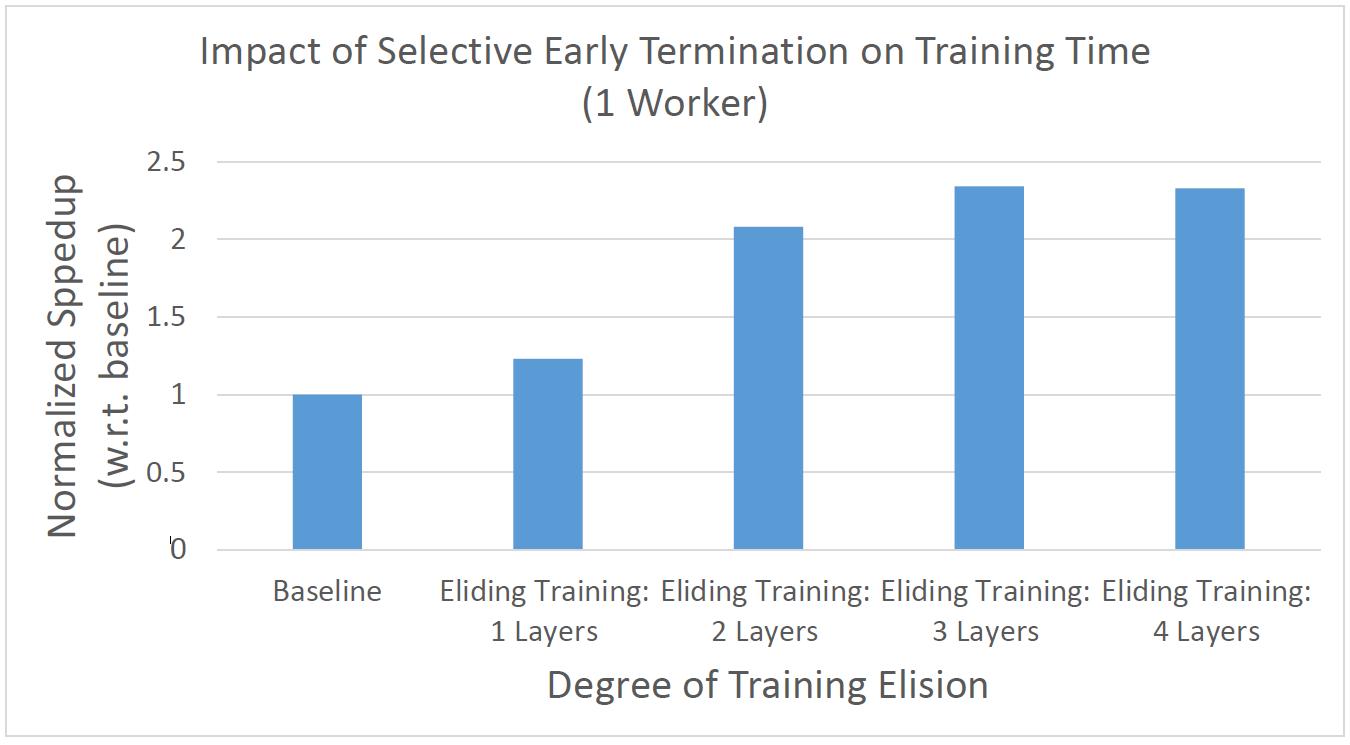
\includegraphics[width=0.8\columnwidth]{figures/fig7.PNG}
	\caption{Normalized speedup for Selective Early Termination: 1 worker}
	\label{fig:fig7}
\end{figure}
%Figure 6: Selective Early Termination (5K steps) -- Accuracy
%Figure 7: Selective Early Termination (5K steps) -- Execution Time
\subsubsection{Multiple Workers Accuracy and Speedups}

\begin{figure}[t]
	\centering
	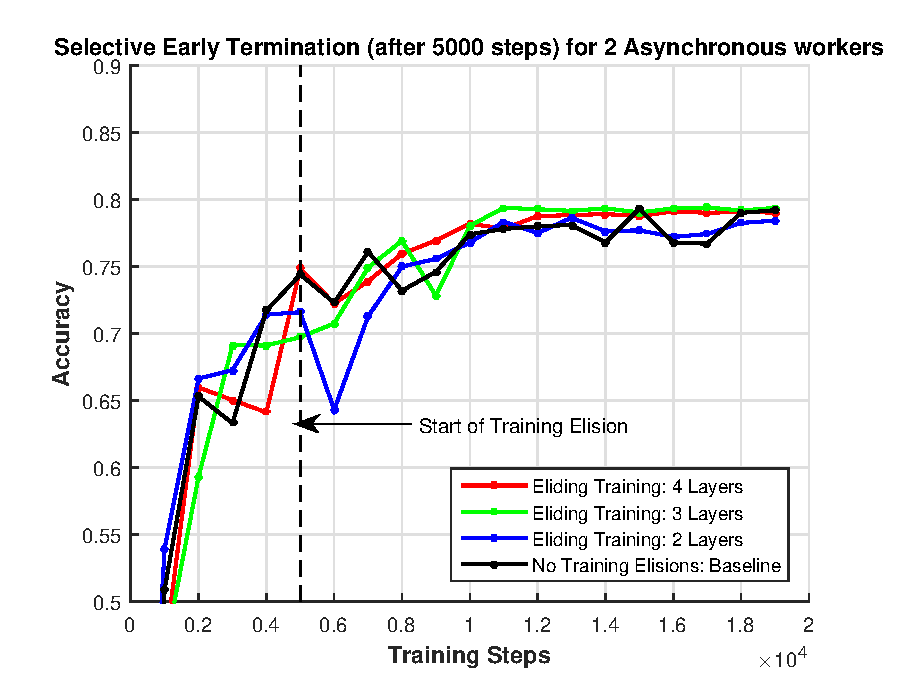
\includegraphics[width=0.8\columnwidth]{figures/fig8.eps}
	\caption{Selective Early Termination for 2 workers (after 5K steps)}
	\label{fig:fig8}
\end{figure}
\begin{figure}[t]
	\centering
	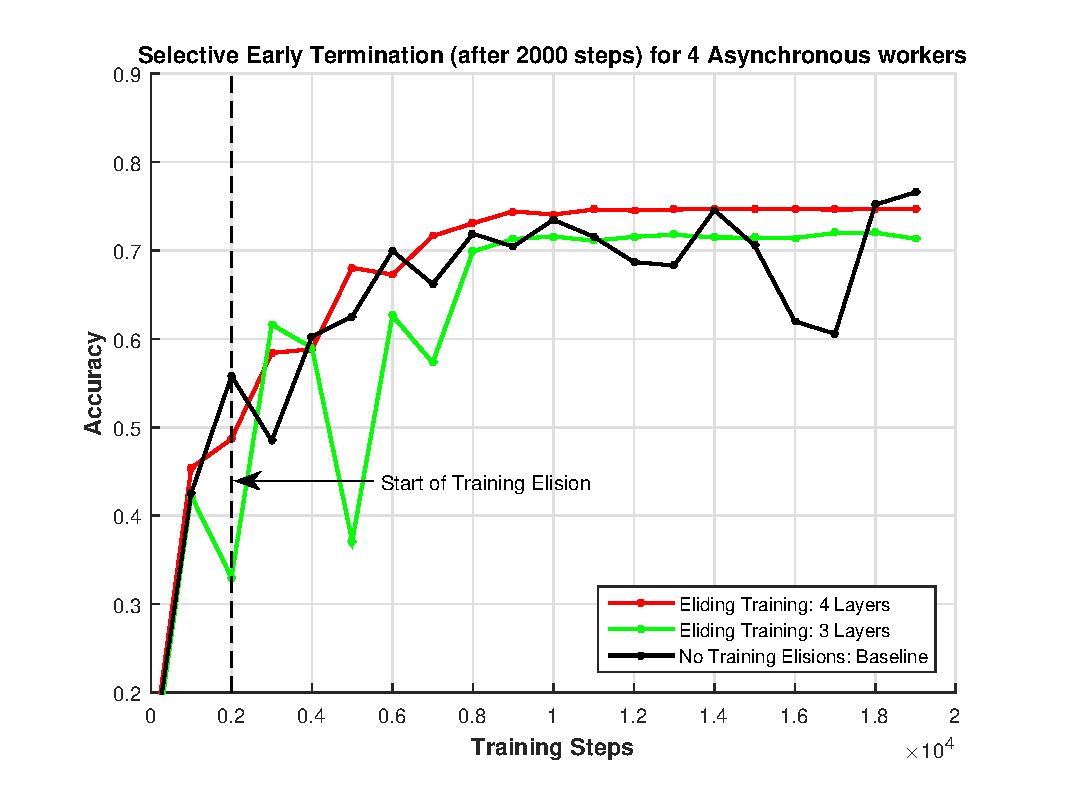
\includegraphics[width=0.8\columnwidth]{figures/fig9.eps}
	\caption{Selective Early Termination for 4 workers (after 2K steps)}
	\label{fig:fig9}
\end{figure}
\begin{figure}[t]
	\centering
	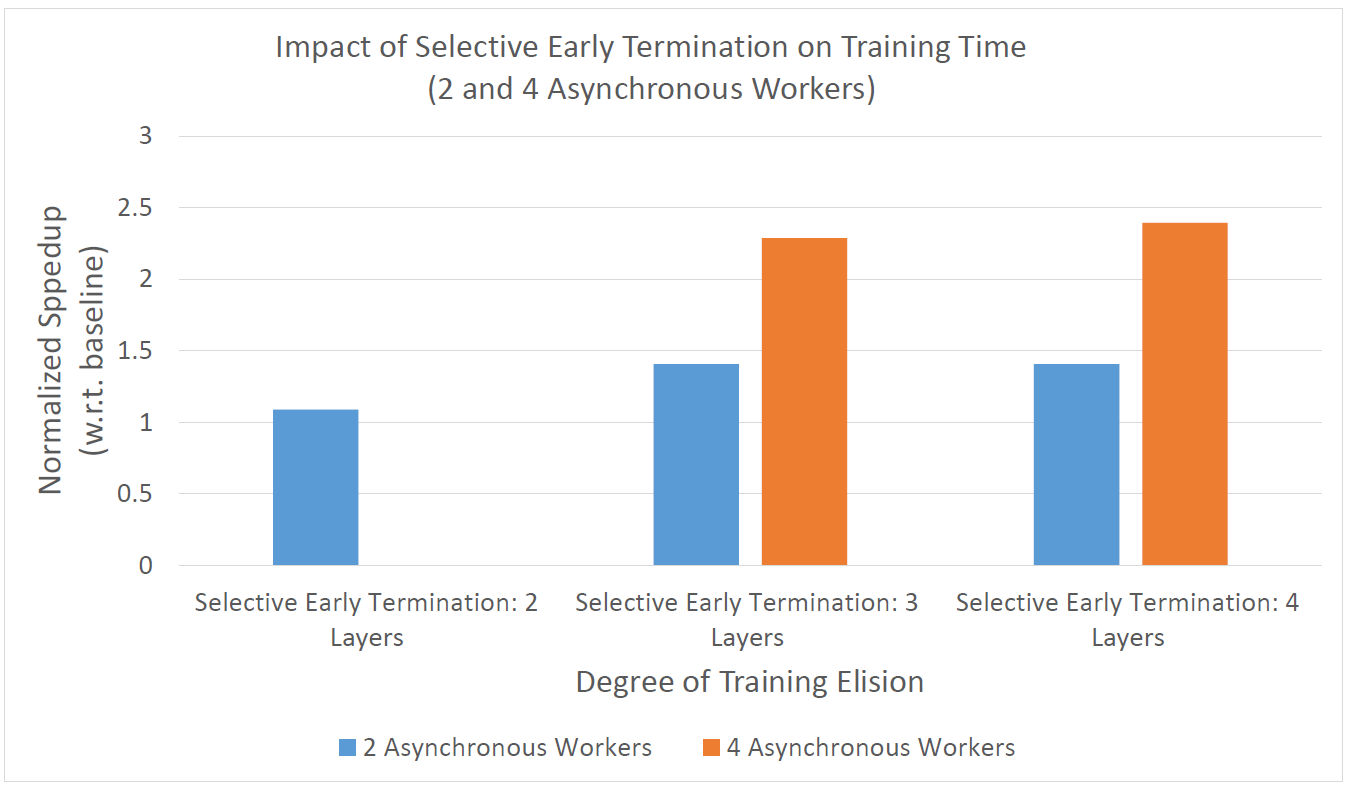
\includegraphics[width=0.8\columnwidth]{figures/fig10.PNG}
	\caption{Normalized speedup for Selective Early Termination: 2 and 4 workers}
	\label{fig:fig10}
\end{figure}
%Figure 8: Selective Early Termination 2 workers (5K steps) -- Accuracy 
%Figure 9: Selective Early Termination 4 workers (2K steps) -- Accuracy
%Figure 10: Selective Early Termination 2 \& 4 (2K \& 5K steps) -- Execution Time


\section{Related Works}

In this section, we compare our work with prior research
on application specific consistency models, distributed
machine learning frameworks and approximating connections 
of deep neural networks.

\emph{\textbf{Data consistency}} There has been considerable
research in relaxed consistency models to improve performance
of distributed machine learning deployments \cite{ganger}\cite{stalesynchronousps}\cite{garth}\cite{parameterserver}.
The proposed solutions vary from performing an empirical study on the 
convergence of different parameter server consistency model\cite{garth}, 
heuristics to bound the amount of staleness \cite{ganger} to 
allowing the programmer to specify the required consistency model \cite{parameterserver}.
Our work takes the same direction as these prior work, by exploring
relaxed consistency models for improved performance. However, we take
a different approach from these works because we use application specific
hints to understand the effect of approximation on different layers of a 
deep neural network.

\emph{\textbf{Distributed Machine Learning Frameworks}} There are many
machine learning frameworks that allow distributed machine learning \cite{tensorflow}
\cite{parameterserver}\cite{distbelief}\cite{petuum}\cite{mxnet}. The sheer number
of these frameworks indicates the importance of distributing machine learning
applications across multiple machines. We expect our approximation strategies
to be applicable generally across different frameworks.

\emph{\textbf{Approximating network connections}} Recent work has explored 
compressing deep neural network to reduce the storage overhead of storing 
model parameters \cite{compresseddnn}\cite{eie}. These works rely on techniques
such as reducing the floating point precision of network weights and pruning
the connections from a fully connected network. While the general idea of 
exploiting the network structures to optimize performance and size of the network
is similar to our work, the main difference is that these works solely focus on 
the problem of inference. It would be interesting to study whether the proposed
techniques would work for the problem of network training.

 




\section{Conclusion}
\subsection{Learnings:}
\subsection{Contributions:}
\begin{itemize}
\item An analysis of the scalability of distributed training using TensorFlow
\item An evaluation of heterogeneous approximation techniques to accelerate distributed training
\end{itemize}
\subsection{Constraints:}


\bstctlcite{bstctl:etal, bstctl:nodash, bstctl:simpurl}
\bibliographystyle{IEEEtranS}
\bibliography{references}

\end{document}

